%%%%%%%%%%%%%%%%%%%%%%%%%%%%%%%%%%%%%%%%%
% Wenneker Assignment
% LaTeX Template
% Version 2.0 (12/1/2019)
%
% This template originates from:
% http://www.LaTeXTemplates.com
%
% Authors:
% Vel (vel@LaTeXTemplates.com)
% Frits Wenneker
%
% License:
% CC BY-NC-SA 3.0 (http://creativecommons.org/licenses/by-nc-sa/3.0/)
% 
%%%%%%%%%%%%%%%%%%%%%%%%%%%%%%%%%%%%%%%%%

%----------------------------------------------------------------------------------------
%	PACKAGES AND OTHER DOCUMENT CONFIGURATIONS
%----------------------------------------------------------------------------------------

\documentclass[11pt]{scrartcl} % Font size

%%%%%%%%%%%%%%%%%%%%%%%%%%%%%%%%%%%%%%%%%
% Wenneker Assignment
% Structure Specification File
% Version 2.0 (12/1/2019)
%
% This template originates from:
% http://www.LaTeXTemplates.com
%
% Authors:
% Vel (vel@LaTeXTemplates.com)
% Frits Wenneker
%
% License:
% CC BY-NC-SA 3.0 (http://creativecommons.org/licenses/by-nc-sa/3.0/)
% 
%%%%%%%%%%%%%%%%%%%%%%%%%%%%%%%%%%%%%%%%%

%----------------------------------------------------------------------------------------
%	PACKAGES AND OTHER DOCUMENT CONFIGURATIONS
%----------------------------------------------------------------------------------------

\usepackage{amsmath, amsfonts, amsthm} % Math packages

\usepackage{listings} % Code listings, with syntax highlighting

\usepackage{xcolor} % Color extensions

\usepackage{cleveref} % Smarter referencing to labels {figures, tables, etc...}
\crefname{lstlisting}{listing}{listings}
\Crefname{lstlisting}{Listing}{Listings}

\usepackage[english]{babel} % English language hyphenation

\usepackage{graphicx} % Required for inserting images
\graphicspath{{graphics/}{./}} % Specifies where to look for included images (trailing slash required)

\usepackage{booktabs} % Required for better horizontal rules in tables

\usepackage{parskip} % Automatically insert newline

\usepackage{multirow} % allows multiple row in tabular environment

\numberwithin{equation}{section} % Number equations within sections (i.e. 1.1, 1.2, 2.1, 2.2 instead of 1, 2, 3, 4)
\numberwithin{figure}{section} % Number figures within sections (i.e. 1.1, 1.2, 2.1, 2.2 instead of 1, 2, 3, 4)
\numberwithin{table}{section} % Number tables within sections (i.e. 1.1, 1.2, 2.1, 2.2 instead of 1, 2, 3, 4)

\setlength\parindent{0pt} % Removes all indentation from paragraphs

\usepackage{enumitem} % Required for list customisation
\setlist{noitemsep} % No spacing between list items

%----------------------------------------------------------------------------------------
%	DOCUMENT MARGINS
%----------------------------------------------------------------------------------------

\usepackage{geometry} % Required for adjusting page dimensions and margins

\geometry{
	paper=a4paper, % Paper size, change to letterpaper for US letter size
	top=2.5cm, % Top margin
	bottom=3cm, % Bottom margin
	left=3cm, % Left margin
	right=3cm, % Right margin
	headheight=0.75cm, % Header height
	footskip=1.5cm, % Space from the bottom margin to the baseline of the footer
	headsep=0.75cm, % Space from the top margin to the baseline of the header
	%showframe, % Uncomment to show how the type block is set on the page
}

%----------------------------------------------------------------------------------------
%   Listing Style	
%----------------------------------------------------------------------------------------

\definecolor{ao}{rgb}{0.0, 0.5, 0.0}

\lstdefinestyle{CStyle}{
  language=C,                     % choose the language of the code
  numbers=left,                   % where to put the line-numbers
  stepnumber=1,                   % the step between two line-numbers.        
  numbersep=5pt,                  % how far the line-numbers are from the code
  backgroundcolor=\color{white},  % choose the background color. You must add \usepackage{color}
  commentstyle=\color{ao},
  keywordstyle=\color{blue},
  showspaces=false,               % show spaces adding particular underscores
  showstringspaces=false,         % underline spaces within strings
  showtabs=false,                 % show tabs within strings adding particular underscores
  tabsize=2,                      % sets default tabsize to 2 spaces
  captionpos=b,                   % sets the caption-position to bottom
  breaklines=true,                % sets automatic line breaking
  breakatwhitespace=true,         % sets if automatic breaks should only happen at whitespace
  title=\lstname,                 % show the filename of files included with \lstinputlisting;
}

%----------------------------------------------------------------------------------------
%	FONTS
%----------------------------------------------------------------------------------------

\usepackage[utf8]{inputenc} % Required for inputting international characters
\usepackage[T1]{fontenc} % Use 8-bit encoding

\usepackage{fourier} % Use the Adobe Utopia font for the document

%----------------------------------------------------------------------------------------
%	SECTION TITLES
%----------------------------------------------------------------------------------------

\usepackage{sectsty} % Allows customising section commands

\renewcommand\thesubsection{\alph{subsection}} % Alpha subsection numbering 
\renewcommand\thesubsubsection{\roman{subsubsection}} % roman subsubsection numbering

\sectionfont{\vspace{6pt}\centering\normalfont\scshape} % \section{} styling
\subsectionfont{\normalfont\bfseries} % \subsection{} styling
\subsubsectionfont{\normalfont\itshape} % \subsubsection{} styling
\paragraphfont{\normalfont\scshape} % \paragraph{} styling

%----------------------------------------------------------------------------------------
%	HEADERS AND FOOTERS
%----------------------------------------------------------------------------------------

\usepackage{scrlayer-scrpage} % Required for customising headers and footers

\ohead*{} % Right header
\ihead*{} % Left header
\chead*{} % Centre header

\ofoot*{} % Right footer
\ifoot*{} % Left footer
\cfoot*{\pagemark} % Centre footer
 % Include the file specifying the document structure and custom commands

%----------------------------------------------------------------------------------------
%	TITLE SECTION
%----------------------------------------------------------------------------------------

\title{	
	\normalfont\normalsize
	\textsc{Curtin University, Concurrent Systems}\\ % Your university, school and/or department name(s)
	\vspace{25pt} % Whitespace
	\rule{\linewidth}{0.5pt}\\ % Thin top horizontal rule
	\vspace{20pt} % Whitespace
	{\huge Lab report 3}\\ % The assignment title
	\vspace{12pt} % Whitespace
	\rule{\linewidth}{2pt}\\ % Thick bottom horizontal rule
	\vspace{12pt} % Whitespace
}

\author{\LARGE Nhan Dao} % Your name

\date{\normalsize\today} % Today's date (\today) or a custom date

\begin{document}

\maketitle % Print the title

%----------------------------------------------------------------------------------------
%	Monte Carlo method for estimating Pi using OpenMP
%----------------------------------------------------------------------------------------

\section{Monte Carlo method for approximating the value of $\pi$ in OpenMP}

\subsection{Compile and run the template code with a single thread, and thus verify that the serial
version is correct.}

\begin{figure}[ht]
    \centering
    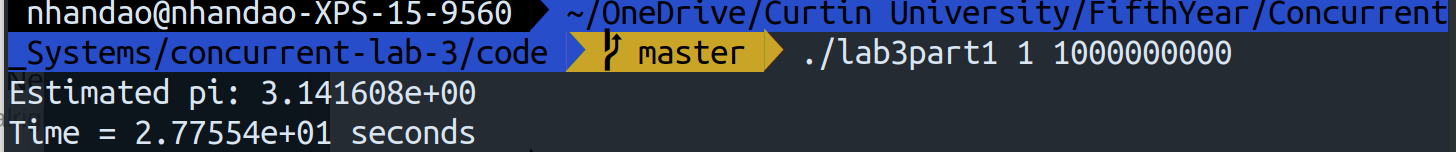
\includegraphics[width=\textwidth]{graphics/P1_a_terminal_output.png}
    \caption{Terminal output of execution of template code with a single thread}
    \label{fig:P1_a_term_out}
\end{figure}

\subsection{Parallelize the code for multi-threaded execution by ONLY adding OpenMP directives}

\vspace{0.5cm}
\lstinputlisting[
	style=CStyle,
	firstline=34, % First line of code
	lastline=48, % Lastl ine of code
	caption=Parallizing the code for multi-threaded execution (line 34-48 in lab3part1.c), % Caption above the listing
	label=lst:lab3part1a, % Label for referencing this listing
	frame=single, % Frame around the code listing
	showstringspaces=false, % Don't put marks in string spaces
	numbers=left, % Line numbers on left
	numberstyle=\normalsize % Line numbers styling
    ]{../code/lab3part1.c}
    
\subsubsection{At what point in the code new threads are forked and joined?}
The code is serial up until \emph{pragma}. At pragma, multiple threads are forked,
line 1 in \cref{lst:lab3part1a}. After the structured block (line 2 - 15), the slaves are joined with 
the master thread and execution resumes on the master thread.

\subsubsection{Which part of the code is executed by which threads?}
The total number of threads are comprised of one main thread, and the remainder are slave threads.
The main thread will run all code outside of the parallel enivornment. Master and slaves thread will 
run the section of code assigned by the OpenMP directives - line 2 - 15.

\subsubsection{Where barrires if any in terms of thread synchronization would be encountered,
and hence how the code achives parallelization}

Thread synchronization is needed to so reduction can be apply to the variable
\emph{number\_in\_circle} to avoid race condition. OpenMP's reduction basically
behaves similarly to a critical section in terms of synchronisation.


\subsection{Tabulate the speedup and efficiency for 1,2,4,8 threads.}

\begin{center}
\begin{tabular}{|| c | c | c | c ||}
	\hline
	Threads & Time (s) & Speedup & Efficiency (\%) \\ [0.5ex]
	\hline 
	1 & 20.356 & N/A & 100 \\
	2 & 10.376 & 1.962 & 98.10 \\
	4 & 5.908 & 3.476 & 86.90 \\
	8 & 3.498 & 5.819 & 72.74 \\
	\hline
\end{tabular}
\end{center}

\begin{figure}[ht]
	\centering
	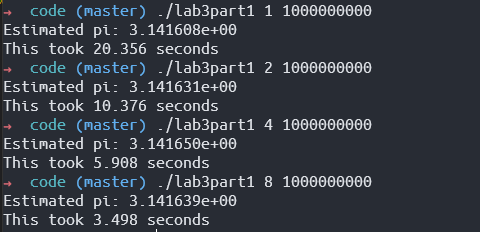
\includegraphics[width=\textwidth]{graphics/P1_c_terminal_output.PNG}
	\caption{Terminal output for execution with 1, 2, 4, 8 threads respectively for
	estimating $pi$ using Monte Carlo's method with $10^9$ samples}
	\label{fig:lab3part1c}
\end{figure}

\subsubsection{Do the result match your expectation? Why?}

The result matches our expectation. The speedup will increase as the number
of threads increase but will saturate at somepoint due to Amdahl's Law which
states that the parallel program is bounded by the section of code that 
can only be executed in serial. Hence, even though we are allocating more
threads, the efficiency decreases and we get a diminishing return due to this
fact. % Monte Carlo's extimation of Pi using POSIX's pthreads	

\end{document}
